\chapter{Metode Penelitian}

\section{Alat dan Bahan Tugas akhir}

\subsection{Alat Tugas akhir}

Pengerjaan penelitian ini menggunakan alat dan bahan. Alat yang digunakan berupa perangkat keras seperti laptop untuk menjalankan program, software, serta library yang 
akan digunakan.

\begin{enumerate}
	\item Laptop MSI GL63 8RD

    Merupakan perangkat keras yang digunakan untuk melakukan implementasi algoritma.
    Laptop ini memiliki spesifikasi sebagai berikut : Sistem operasi Windows 11, {Processor} Intel I7-8750H, Memori 16GB DDR4, NVIDIA GeForce GTX 1050 (4GB), 
    SSD Samsung MZNLN128HAHQ 128GB, dan HDD HGST HTS721010A9E630

    \item Python 3.10
	
    Python adalah bahasa pemrograman utama yang digunakan pada penelitian ini.

	\item Visual Studio Code
	
    Visual Studio Code adalah \textit{source code editor} yang digunakan untuk membantu menulis kode program pada penelitian ini.
	\item Google Colaboratory
	
    Google Colaboratory adalah platform berbasis \textit{cloud computing} yang digunakan untuk menjalankan kode program python pada penelitian ini.
    dengan spesifikasi sebagai berikut: Intel Xeon CPU, RAM 12.72 GB, serta penyimpanan 107.7 GB.

\end{enumerate}


\subsection{Bahan Tugas akhir}

\begin{table}[H]
    \centering
    \begin{tabular}{||p{1em}|p{3em}|p{3em}|p{4em}||}
    \hline
       No & Lebar & Tinggi & Kelas\\ [0.5ex]
        \hline\hline
        1 & 1.1 & 1.3 & lemari\\ \hline 
        2 & 1.1 & 1.5 & lemari\\ \hline	
        3 & 0.7 & 1.5 & lemari\\ \hline	
        4 & 0.6 & 1.9 & lemari\\ \hline	
        5 & 0.8 & 2 & lemari\\ \hline	
        6 & 1.2 & 0.6 & buffet\\ \hline	
        7 & 1.6 & 0.5 & buffet\\ \hline	
        8 & 1.7 & 0.7 & buffet\\ \hline	
        9 & 2.2 & 0.4 & buffet\\ \hline	
        10 & 2.2 & 0.5 & buffet\\ \hline	
        11 & 2.3 & 0.8 & buffet\\ \hline	
        12 & 1.5 & 0.5 & buffet\\ \hline
        13 & 2 & 2 & wardrobe\\ \hline
        14 & 1.8 & 2.2 & wardrobe\\ \hline	
        15 & 1.5 & 1.8 & wardrobe\\ \hline	
        16 & 2.3 & 1.5 & wardrobe\\ \hline
        \end{tabular}
    \caption{Dataset ukuran lebar dan tinggi dari lemari, buffet, dan wardrobe}
    \label{tab:Dataset}
\end{table}

Dataset dapat dilihat pada Tabel \ref{tab:Dataset}. 
Dataset yang digunakan berupa data tinggi dan lebar suatu lemari, \textit{buffet}, dan \textit{wardrobe}. 
Kelas lemari terdiri dari lima data dengan lebar berkisar  antara 0.6 hingga 1.1 dan tinggi berkisar antara 1.3 hingga 2.0.
Kelas buffet terdiri dari tujuh data dengan karakteristik lebar yang relatif lebih besar, yaitu antara 1.2 hingga 2.3, namun memiliki tinggi yang lebih rendah, 
berkisar antara 0.5 hingga 2.0.
Sementara itu, kelas wardrobe terdiri dari empat data terakhir dengan lebar antara 1,5 hingga 2,3 dan tinggi antara 1,5 hingga 2,2.

\begin{figure}[H]
    \centering
    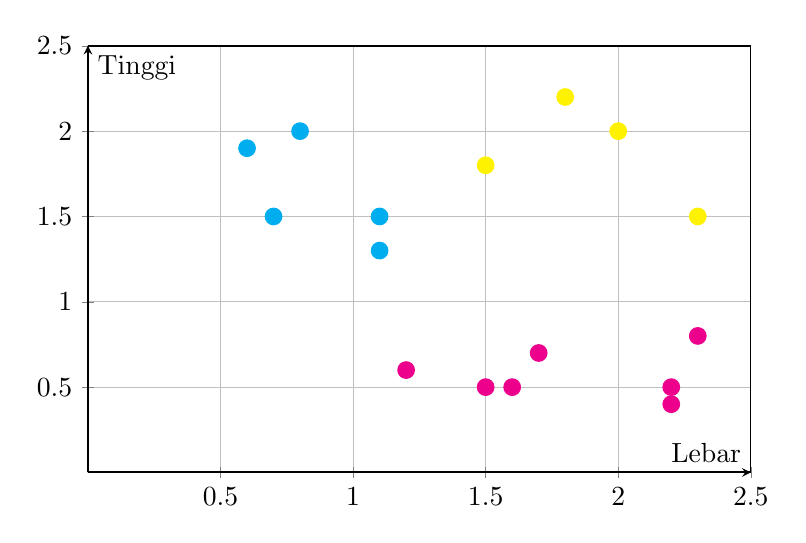
\begin{tikzpicture}
        \begin{axis}[
            xlabel=Lebar,
            ylabel=Tinggi,
            xmin=0, xmax=2.5,
            ymin=0, ymax=2.5,
            width=10cm,
            height=7cm,
            domain=-4:4,
            grid=both,
            samples=100,
            legend pos=south west,
            axis lines=middle, % Add this line to get the axes in the middle
        ]

        % Adding points
        \addplot[mark=*, color=cyan, mark size = 3] coordinates {(1.1,1.3)};
        \addplot[mark=*, color=cyan, mark size = 3] coordinates {(1.1,1.5)};
        \addplot[mark=*, color=cyan, mark size = 3] coordinates {(0.7,1.5)};
        \addplot[mark=*, color=cyan, mark size = 3] coordinates {(0.6,1.9)};
        \addplot[mark=*, color=cyan, mark size = 3] coordinates {(0.8,2)};
        \addplot[mark=*, color=magenta, mark size = 3] coordinates {(1.2,0.6)};
        \addplot[mark=*, color=magenta, mark size = 3] coordinates {(1.6,0.5)};
        \addplot[mark=*, color=magenta, mark size = 3] coordinates {(1.7,0.7)};
        \addplot[mark=*, color=magenta, mark size = 3] coordinates {(2.2,0.4)};
        \addplot[mark=*, color=magenta, mark size = 3] coordinates {(2.2,0.5)};
        \addplot[mark=*, color=magenta, mark size = 3] coordinates {(2.3,0.8)};
        \addplot[mark=*, color=magenta, mark size = 3] coordinates {(1.5,0.5)};
        \addplot[mark=*, color=yellow, mark size = 3] coordinates {(2,2)};
        \addplot[mark=*, color=yellow, mark size = 3] coordinates {(1.8,2.2)};
        \addplot[mark=*, color=yellow, mark size = 3] coordinates {(1.5,1.8)};
        \addplot[mark=*, color=yellow, mark size = 3] coordinates {(2.3,1.5)};


        % Draw frame
        \draw[black, thick] (rel axis cs:0,0) rectangle (rel axis cs:1,1);
        \end{axis}
    \end{tikzpicture}
    \caption{Grafik dari dataset pada Tabel \ref{tab:Dataset}}
    \label{fig:plot dataset}
\end{figure}

Gambar \ref{fig:plot dataset} memperlihatkan grafik sebaran dari dataset pada Tabel \ref{tab:Dataset} dengan sumbu horizontal menunjukkan Lebar dan sumbu vertikal menunjukkan Tinggi. 
Setiap titik merepresentasikan satu data furnitur, sedangkan perbedaan warna menunjukkan kelas yang berbeda. Terlihat bahwa data membentuk tiga kelompok yang cukup jelas. 
Titik berwarna \textit{Cyan} adalah lemari, \textit{magenta} adalah buffet, dan kuning adalah wardrobe
Kelompok dengan tinggi relatif besar dan lebar kecil berada di sisi kiri atas grafik, yang merepresentasikan kelas lemari. Kelompok dengan lebar besar namun tinggi rendah terkonsentrasi di bagian bawah kanan grafik, yang menunjukkan kelas buffet. 
Sementara itu, kelas wardrobe berada pada area dengan nilai lebar dan tinggi yang sama-sama relatif besar, yaitu di bagian kanan atas grafik. 
Pola ini menunjukkan bahwa \textit{feature} lebar dan tinggi mampu membedakan kelas furnitur secara visual.

\section{Metode yang Digunakan}

Penelitian ini menggunakan pendekatan \textit{kuantitatif} untuk menganalisis pengaruh jumlah \textit{hidden layer} terhadap akurasi dan waktu komputasi pada jaringan saraf tiruan. 
Penelitian ini dilakukan dengan mengembangkan beberapa model jaringan saraf tiruan. 
Seluruh proses pengembangan dan pelatihan model diimplementasikan menggunakan bahasa pemrograman \textit{Python} versi 3.10.
Setelah berhasil dikembangkan, dilakukan pencarian parameter yang paling optimal untuk model tersebut.
Sebelum proses pelatihan, dataset diproses terlebih dahulu menggunakan metode normalisasi. 
Data ternormalisasi akan digunakan dalam proses pencarian parameter optimal dan pelatihan model. 

Untuk menganalisis pengaruh jumlah \textit{hidden layer}, jaringan saraf tiruan dibangun dengan beberapa konfigurasi arsitektur yang berbeda. 
Terdapat tiga model utama yang digunakan, yaitu:
\begin{enumerate}
    \item Model pertama model dengan satu \textit{hidden layer} dan jumlah \textit{neuron} yang bervariasi.
    \item Model kedua model dengan beberapa \textit{hidden layer} dengan jumlah \textit{neuron} yang sama pada setiap \textit{hidden layer}.
\end{enumerate}

Evaluasi kinerja model dilakukan dengan mengukur nilai akurasi dan waktu pelatihan, yang selanjutnya dianalisis menggunakan statistik deskriptif dan uji signifikansi.

\subsection{Implementasi Algoritma Pelatihan}

Algoritma pelatihan dengan metode \textit{backpropagation}.
Nilai gradient akan didapatkan dari metode \textit{backpropagation}. 
Nilai gradient akan digunakan untuk menentukan arah perubahan bobot.
Perubahan bobot dilakukan dengan metode \textit{newthon raphson} seperti pada Persamaan [ubah]
Perubahan bobot dilakukan satu persatu hingga didapatkan perubahan \textit{relative} bobot baru dengan bobot lama kurang dari 0.1.
Kemudian dilanjutkan dengan bobot selanjutnya hingga semua bobot dan bias pada layer tersebut telah diperbarui.

\begin{algorithm}
	\caption{Algoritma Pelatihan}\label{alg: Pelatihan}
	\begin{algorithmic}[1]
        \Function{InitializeWeightsandBiases}{$TotalLayer$}
            \For {each $l$ in $TotalLayer$}
                \State $\mathbf{W}^{l} \gets$ Generate Random matrix 
            \EndFor
            \State \Return $\mathbf{W}$
        \EndFunction \\

        \Function{ForwardPropagation}{$\mathbf{X}, TotalLayer$}
            \For {each $l$ in $TotalLayer$}
                \State $\mathbf{Y}^{l} \gets \mathbf{W}^{l} \cdot \mathbf{X}^{l-1}$
                \State $\mathbf{X}^{l} \gets$ $\mathbf{Y}^{l}$
            \EndFor
            \State \Return $\mathbf{Y}^{L}$
        \EndFunction \\

        \Function{CalculateGradient}{$TotalLayer$}
            \State $\frac{dJ}{dY} \gets (-2/m) * (y - \hat{y})$
            \For {each $l$ in $TotalLayer$}
                \If {$l = L$}
                    \State $\delta \gets \frac{dJ}{dY}$
                \EndIf
                \If {$l \neq L$}
                    \State $\delta \gets w^{l+1} \cdot \delta$
                \EndIf
                \State $\frac{dJ}{dw^{l}} \gets \delta \cdot x^{l-1}$
                \EndFor
            \State \Return $\frac{dJ}{dw}$
        \EndFunction \\

        % \Function{RelativeWeightChange}{$w_{new}, w^{l}_{i}$}
        %     \State $e \gets \frac{|w_{new} - w^{l}_{i}|}{|w^{l}_{i}|}$
        %     \State \Return $e$
        % \EndFunction \\

        % \Function{Backpropagation}{$ExpectedValue$}
        %     \For {each $l$ in TotalLayer}
        %         \For {each $i$ in $W^{l}$}
        %             \While {$e < 0.1$}
        %                 \State $\frac{J'}{J''}$ $\gets$ CalculateGradient()
        %                 \State $w_{new} \gets$ $w^{l}_{i} - \eta \cdot \frac{J'}{J''}$
        %                 \State $e \gets$ RelativeWeightChange ($w_{new}, w^{l}_{i}$)
        %             \EndWhile
        %         \EndFor 
        %     \EndFor
        % \EndFunction \\

        % \Function{TrainModel}{$InputData, ExpectedValue, TotalLayer, Epoch$}
        %     \State $epoch \gets 0$
        %     \State $\mathbf{W} \gets$ InitializeWeightsandBiases($TotalLayer$)
        %     \While {$epoch \neq Epoch$ or $\alpha \neq 0$}
        %         \State $y^{L} \gets$ ForwardPropagation($InputData$)
        %         \State Backpropagation($ExpectedValue$)
        %         \State $\alpha \gets y-\hat{y}$ 
        %         \State $epoch \gets epoch + 1$
        %     \EndWhile
        % \EndFunction \\
        \algstore{RelativeWeightChange}
	\end{algorithmic}
\end{algorithm}


\begin{algorithm}
	\begin{algorithmic}[1]
        \algrestore{RelativeWeightChange}
        \Function{RelativeWeightChange}{$w_{new}, w^{l}_{i}$}
            \State $e \gets \frac{|w_{new} - w^{l}_{i}|}{|w^{l}_{i}|}$
            \State \Return $e$
        \EndFunction \\

        \Function{Backpropagation}{$ExpectedValue$}
            \For {each $l$ in TotalLayer}
                \For {each $i$ in $W^{l}$}
                    \While {$e < 0.1$}
                        \State $\frac{J'}{J''}$ $\gets$ CalculateGradient()
                        \State $w_{new} \gets$ $w^{l}_{i} - \eta \cdot \frac{J'}{J''}$
                        \State $e \gets$ RelativeWeightChange ($w_{new}, w^{l}_{i}$)
                    \EndWhile
                \EndFor 
            \EndFor
        \EndFunction \\

        \Function{TrainModel}{$InputData, ExpectedValue, TotalLayer, Epoch$}
            \State $epoch \gets 0$
            \State $\mathbf{W} \gets$ InitializeWeightsandBiases($TotalLayer$)
            \While {$epoch \neq Epoch$ or $\alpha \neq 0$}
                \State $y^{L} \gets$ ForwardPropagation($InputData$)
                \State Backpropagation($ExpectedValue$)
                \State $\alpha \gets y-\hat{y}$ 
                \State $epoch \gets epoch + 1$
            \EndWhile
        \EndFunction \\
	\end{algorithmic}
\end{algorithm}

Parameter yang digunakan pada algoritma pelatihan ini adalah sebagai berikut:

\begin{enumerate}[label=(\alph*)]
    \item $\eta$ adalah learning rate
    \item $TotalLayer$ adalah jumlah \textit{hidden layer} yang digunakan
    \item $Epoch$ adalah jumlah pengulangan pelatihan yang dilakukan
\end{enumerate}

\subsection{\textit{Dataset} yang digunakan}

% Dataset yang digunakan adalah data tinggi dan lebar suatu \textit{furniture} beserta kategorinya.
Dataset dapat dilihat pada Tabel \ref{tab:Dataset}. 
Dataset terdiri dari 16 \textit{instance} dengan dua \textit{feature} yaitu lebar dan tinggi serta 3 kelas yaitu lemari, buffet, dan wardrobe.
Plot dari dataset dapat dilihat pada Gambar \ref{fig:plot dataset}.
Data ini tidak langsung digunakan namun diolah terlebih dahulu dengan normalisasi.

\subsection{Desain Eksperimen}

Dilakukan pengujian performa pada kode hasil implementasi algoritma pelatihan pada dataset tinggi dan lebar suatu lemari, buffet, dan wardrobe.
Detail dari eksperimen yang dilakukan adalah sebagai berikut:

\begin{enumerate}
    \item \textbf{Normalisasi Data}
    
    Data pada Tabel \ref{tab:Dataset} akan di normalisasikan dengan metode \textit{Minmax Scaling}.
    Data tersebut juga akan diberikan label agar dapat digunakan pada algoritma \textit{supervised learning}.

    \begin{table}[H]
        \centering
        \begin{tabular}{||p{1em}|p{3em}|p{3em}|p{2em}|p{2em}|p{2em}||}
        \hline
            No & Lebar & Tinggi & $C_0$ & $C_1$ & $C_2$\\ [0.5ex]
            \hline
            1 & 0.36 & 0.47 & 1 & -1 & -1\\ \hline 
            2 & 0.36 & 0.57 & 1 & -1 & -1\\ \hline	
            3 & 0.15 & 0.57 & 1 & -1 & -1\\ \hline	
            4 & 0.10 & 0.78 & 1 & -1 & -1\\ \hline	
            5 & 0.21 & 0.83 & 1 & -1 & -1\\ \hline	
            6 & 0.41 & 0.10 & -1 & 1 & -1\\ \hline	
            7 & 0.62 & 0.05 & -1 & 1 & -1\\ \hline	
            8 & 0.67 & 0.15 & -1 & 1 & -1\\ \hline	
            9 & 0.93 & 0.00 & -1 & 1 & -1\\ \hline	
            10 & 0.93 & 0.05 & -1 & 1 & -1\\ \hline	
            11 & 0.99 & 0.21 & -1 & 1 & -1\\ \hline	
            12 & 0.57 & 0.05 & -1 & 1 & -1\\ \hline
            13 & 0.83 & 0.83 & -1 & -1 & 1\\ \hline
            14 & 0.73 & 0.93 & -1 & -1 & 1\\ \hline	
            15 & 0.57 & 0.57 & -1 & -1 & 1\\ \hline	
             16 & 0.99 & 0.57 & -1 & -1 & 1\\ \hline
        \end{tabular}
        \caption{Dataset ukuran lebar dan tinggi dari lemari, buffet, dan wardrobe setelah normalisasi dan pemberian label}
        \label{tab:Dataset normalisasi}
    \end{table}

    Tabel \ref{tab:Dataset normalisasi} menunjukan dataset setelah dilakukan normalisasi dengan metode \textit{Minmax Scaling} dan pemberian label.
    Setiap baris merepresentasikan satu objek dengan rentang nilai 0 hingga 1, sehingga perbedaan skala antar \textit{feature} dapat diminimalkan.
    Kemudian pemberian kelas $C_0$, $C_1$, dan $C_2$ dengan skema pengkodean bernilai $1$ dan $-1$. 
    Nilai 1 menunjukkan keanggotaan data pada kelas tertentu, sedangkan nilai $-1$ menunjukkan bahwa data tersebut tidak termasuk dalam kelas tersebut.

    \begin{figure}[H]
        \centering
        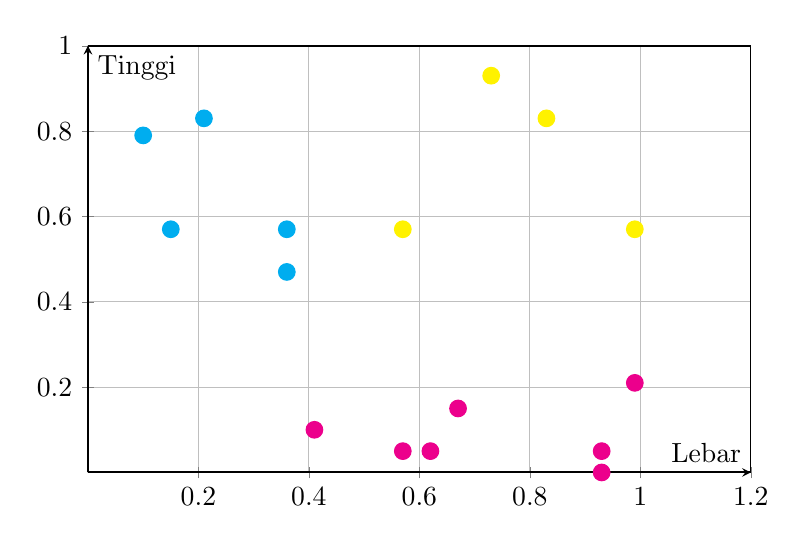
\begin{tikzpicture}
            \begin{axis}[
                xlabel=Lebar,
                ylabel=Tinggi,
                xmin=0, xmax=1.2,
                ymin=0, ymax=1,
                width=10cm,
                height=7cm,
                domain=-4:4,
                grid=both,
                samples=100,
                legend pos=south west,
                axis lines=middle, % Add this line to get the axes in the middle
            ]

            % Adding points
            \addplot[mark=*, color=cyan, mark size = 3] coordinates {(0.36,0.47)};
            \addplot[mark=*, color=cyan, mark size = 3] coordinates {(0.36,0.57)};
            \addplot[mark=*, color=cyan, mark size = 3] coordinates {(0.15,0.57)};
            \addplot[mark=*, color=cyan, mark size = 3] coordinates {(0.10,0.79)};
            \addplot[mark=*, color=cyan, mark size = 3] coordinates {(0.21,0.83)};
            \addplot[mark=*, color=magenta, mark size = 3] coordinates {(0.41,0.10)};
            \addplot[mark=*, color=magenta, mark size = 3] coordinates {(0.62,0.05)};
            \addplot[mark=*, color=magenta, mark size = 3] coordinates {(0.67,0.15)};
            \addplot[mark=*, color=magenta, mark size = 3] coordinates {(0.93,0.00)};
            \addplot[mark=*, color=magenta, mark size = 3] coordinates {(0.93,0.05)};
            \addplot[mark=*, color=magenta, mark size = 3] coordinates {(0.99,0.21)};
            \addplot[mark=*, color=magenta, mark size = 3] coordinates {(0.57,0.05)};
            \addplot[mark=*, color=yellow, mark size = 3] coordinates {(0.83,0.83)};
            \addplot[mark=*, color=yellow, mark size = 3] coordinates {(0.73,0.93)};
            \addplot[mark=*, color=yellow, mark size = 3] coordinates {(0.57,0.57)};
            \addplot[mark=*, color=yellow, mark size = 3] coordinates {(0.99,0.57)};


            % Draw frame
            \draw[black, thick] (rel axis cs:0,0) rectangle (rel axis cs:1,1);
            \end{axis}
        \end{tikzpicture}
        \caption{Grafik dari dataset setelah melalui Minmax Scaling. \textit{Cyan} adalah lemari, \textit{magenta} adalah buffet, dan kuning adalah wardrobe}
        \label{fig:plot dataset normalisasi}
    \end{figure}

    Dari Gambar \ref{fig:plot dataset normalisasi} terlihat bahwa proses normalisasi tidak mengubah pola sebaran data, tetapi hanya menyesuaikan skala nilainya sehingga seluruh fitur berada pada rentang yang sama. 

    \item \textbf{Pencarian Parameter Optimal untuk pelatihan}
    
    Pencarian nilai optimal untuk parameter dilakukan dengan menggunakan metode grid search pada beberapa kandidat parameter.
    Masing-masing kandidat parameter diuji performa waktu komputasinya pada data. 
    Berikut kandidat parameter pada eksperimen pencarian parameter optimal menggunakan grid search:
    \begin{enumerate}[label=(\alph*)]
        \item \textit{Learning rate}
        
        Kemungkinan jumlah iterasi yang digunakan adalah 0.1, 0.2, 0.3, 0.4, 0.5, 0.6, 0.7, 0.8, 0.9, dan 1.0.

        \item Metode optimasi
        
        Kemungkinan metode optimasi yang digunakan adalah tanpa optimasi (\textit{default}), momentum, rmsprop, adagrad, dan adam.
    
    \end{enumerate}

    Pencarian parameter dilakukan dengan melakukan eksperimen sebanyak 30 kali pada dataset ternormalisasi. 
    Jumlah \textit{hidden layer} yang digunakan berkisar satu hingga tiga \textit{hidden layer} dengan jumlah neuron pada setiap \textit{hidden layer} sebanyak empat neuron.
    Pada setiap eksperimen, dilakukan inisialisasi bobot yang berbeda-beda.
    \textit{Random generator} akan menghasilkan nilai random pada rentang interval $(0, 1]$
    Kombinasi parameter yang memilik rata-rata RMSE terkecil pada data uji dari 30
    eksperimen tersebut kemudian dipilih sebagai parameter optimal.

    \item \textbf{Satu hidden layer dan jumlah neuron yang bervariasi}
    
    Setelah mendapatkan parameter optimal, Eksperimen dilakukan dengan variasi jumlah neuron pada satu \textit{hidden layer}.
    Jumlah neuron yang digunakan adalah 2 hingga 40 neuron.
    Metrik yang digunakan untuk evaluasi adalah \textit{epoch} untuk waktu komputasi dan akurasi.
    Prosedur yang dilakukan adalah sebagai berikut:
    \begin{enumerate}[label=(\alph*)]
        \item Eksperimen dilakukan sebanyak 30 kali pada setiap variasi jumlah neuron.
        \item Setiap eksperimen dilakukan dengan \textit{random generator} untuk menghasilkan nilai random pada rentang interval $(0, 1]$
        \item Jumlah \textit{hidden layer} yang digunakan adalah satu dengan variasi jumlah neuron dengan rentang 2 hingga 40.
        \item Pelatihan dilakukan sebanyak maksimal 50000 \textit{epoch} atau berhenti jika nilai error mencapai nol.
        \item Dilakukan perhitungan rata-rata akurasi dan waktu komputasi dari 30 eksperimen pada setiap variasi jumlah neuron.
    \end{enumerate}


    \item \textbf{Beberapa hidden layer dan jumlah neuron yang bervariasi}
    
    Eksperimen dilakukan dengan variasi \textit{hidden layer} dengan jumlah neuron yang tetap pada setiap \textit{hidden layer}.
    Jumlah neuron dipilih dari hasil eksperimen pada poin sebelumnya. 
    Jumlah \textit{hidden layer} yang digunakan adalah 1 hingga 20 \textit{hidden layer}.
    Metrik yang digunakan untuk evaluasi adalah \textit{epoch} untuk waktu komputasi dan akurasi.
    Prosedur yang dilakukan adalah sebagai berikut:
    \begin{enumerate}[label=(\alph*)]
        \item Eksperimen dilakukan sebanyak 30 kali pada setiap variasi jumlah neuron.
        \item Setiap eksperimen dilakukan dengan \textit{random generator} untuk menghasilkan nilai random pada rentang interval $(0, 1]$
        \item Jumlah \textit{hidden layer} yang digunakan adalah 1 hingga 40 \textit{hidden layer} dengan jumlah neuron yang sama.
        \item Pelatihan dilakukan sebanyak maksimal 50000 \textit{epoch} atau berhenti jika nilai error mencapai nol.
        \item Dilakukan perhitungan rata-rata akurasi dan waktu komputasi dari 30 eksperimen pada setiap variasi jumlah neuron.
    \end{enumerate}
\end{enumerate}

\section{Alur Tugas Akhir}

Penelitian ini dilakukan secara bertahap dengan alur seperti pada Gambar \ref{alur_penelitian}.
Studi literatur dilakukan pada awal penelitian untuk memahami konsep dan teori yang akan digunakan pada penelitian. Selanjutnya, dilakukan Pengembangan program jaringan syaraf tiruan dengan bahasa pemrograman python pada \textit{google colaboratory}. Setelah program dibuat, maka dilakukan pengujian untuk mengetahui apakah program berhasil atau tidak. Penelitian diakhiri dengan pengambilan data pengujian dan penyusunan laporan akhir.

\begin{figure}[H]
	\centering
	\resizebox{0.35\textwidth}{!}{%
		\tikzstyle{startstop} = [rectangle, rounded corners, minimum width=3cm, minimum height=1cm, text centered, draw=black, fill=red!30]
		\tikzstyle{analyze} = [rectangle, text width=5cm, minimum width=3cm, minimum height=1cm, text centered, draw=black, fill=orange!30]
		\tikzstyle{process} = [rectangle, text width=5cm, minimum width=3cm, minimum height=1cm, text centered, draw=black, fill=orange!30]
		\tikzstyle{decision} = [diamond, text width=1.5cm, minimum width=1cm, minimum height=1cm, text centered, draw=black, fill=green!30]
		\tikzstyle{arrow} = [thick,->,>=stealth]
		\begin{tikzpicture}[node distance=2cm]
			\node (start) [startstop] {Mulai};
			\node (input) [analyze, below of=start, yshift=0.5cm] {Studi Literatur};
            \node (process0) [process, below of=input, yshift=0.5cm]{Pemilihan jenis ANN};
            \node (process1) [process, below of=process0, yshift=0.5cm]{Pengembangan MLP dengan python};
			\node (process2) [process, below of=process1, yshift=0.5cm] {Melakukan pengujian model};
			\node (decision) [decision, below of=process2, yshift=-0.2cm] {Berhasil?};
            \node (process3) [process, below of=decision, yshift=-0.4cm] {Mencari Parameter Terbaik};
            \node (process4) [process, below of=process3, yshift=-0.1cm] {Membandingkan Performa Satu \textit{Hidden Layer} dan beberapa \textit{Hidden Layer}};
			\node (stop) [startstop, below of=process4, yshift=-0cm] {Selesai};
			\draw [arrow] (start) -- (input);
			\draw [arrow] (input) -- (process0);
            \draw [arrow] (process0) -- (process1);
			\draw [arrow] (process1) -- (process2);
			\draw [arrow] (process2) -- (decision);
			\draw [arrow] (decision.south) -- node[anchor=west, pos=0.3] {Iya} (process3);
		    \draw [arrow] (decision.west) -- node[anchor=south, pos=0.2] {Tidak} (-4,-8.2) -- (-4,-4.5) -- (process1.west);
            \draw [arrow] (process3) -- (process4);
            \draw [arrow] (process4) -- (stop);
		\end{tikzpicture}%
        }
	\caption{Diagram alir penelitian}
    \label{alur_penelitian}
\end{figure}

\subsection{Studi Literatur}
Studi literatur merupakan tahap awal pada penelitian agar dapat memahami lebih lanjut topik penelitian yang dilakukan. 
Studi literatur dilakukan dengan mengumpulkan materi dan referensi dari berbagai sumber seperti artikel, jurnal penelitian, forum, dan situs web.

\subsection{Pemilihan jenis ANN}
Dari hasil studi literatur, diketahui jaringan syaraf tiruan memiliki beberapa model seperti \textit{Feedforward Neural Network} (FNN), \textit{Convolutional Neural Network} (CNN), dan \textit{Recurrent Neural Network} (RNN).
Model yang dipilih pada penelitian ini adalah \textit{Feedforward Neural Network} atau Multi Layer Perceptron (MLP) karena penggunaan MLP lebih umum dibanding model lain.

\subsection{Pengembangan program MLP dengan python}
Pengembangan program dilakukan pada \textit{Google Colaboratory} dan \textit{Visual Studio Code} dengan menggunakan bahasa pemrograman python. Diagram alir dari program terlihat pada Gambar \ref{alur_penelitian}

\subsection{Implementasi Pelatihan}
Algoritma pelatihan kemudian diimplementasikan dengan menggunakan bahasa pemrograman python.

\subsection{Melakukan Pengujian Model}
Model diuji dengan dataset sederhana kemudian dilakukan pengecekan apakah algoritma yang dijalankan sudah benar atau belum.
Indikasi model sudah benar adalah jika nilai error menurun seiring dengan pelatihan yang dijalankan.

\subsection{Mencari Parameter Terbaik}

Dilakukan eksperimen secara iteratif dengan parameter berbeda-beda pada dataset. 
Parameter yang menghasilkan nilai Epoch terkecil pada dataset kemudian dipilih sebagai parameter terbaik

\subsection{Membandingkan Performa Satu \textit{Hidden Layer} dan beberapa \textit{Hidden Layer}}

Performa pada tiap neuron pada konfigurasi satu \textit{hidden layer} dibandingkan.
neuron dengan nilai epoch terkecil kemudian digunakan pada eksperimen beberapa \textit{hidden layer}.
Performa pada tiap \textit{hidden layer} kemudian dibandingkan.
Performa yang diukur adalah akurasi prediksi rating, efisiensi memori serta waktu komputasi.
